% Options for packages loaded elsewhere
% Options for packages loaded elsewhere
\PassOptionsToPackage{unicode}{hyperref}
\PassOptionsToPackage{hyphens}{url}
\PassOptionsToPackage{dvipsnames,svgnames,x11names}{xcolor}
%
\documentclass[
  italian,
  letterpaper,
  DIV=11,
  numbers=noendperiod]{scrartcl}
\usepackage{xcolor}
\usepackage{amsmath,amssymb}
\setcounter{secnumdepth}{-\maxdimen} % remove section numbering
\usepackage{iftex}
\ifPDFTeX
  \usepackage[T1]{fontenc}
  \usepackage[utf8]{inputenc}
  \usepackage{textcomp} % provide euro and other symbols
\else % if luatex or xetex
  \usepackage{unicode-math} % this also loads fontspec
  \defaultfontfeatures{Scale=MatchLowercase}
  \defaultfontfeatures[\rmfamily]{Ligatures=TeX,Scale=1}
\fi
\usepackage{lmodern}
\ifPDFTeX\else
  % xetex/luatex font selection
\fi
% Use upquote if available, for straight quotes in verbatim environments
\IfFileExists{upquote.sty}{\usepackage{upquote}}{}
\IfFileExists{microtype.sty}{% use microtype if available
  \usepackage[]{microtype}
  \UseMicrotypeSet[protrusion]{basicmath} % disable protrusion for tt fonts
}{}
\makeatletter
\@ifundefined{KOMAClassName}{% if non-KOMA class
  \IfFileExists{parskip.sty}{%
    \usepackage{parskip}
  }{% else
    \setlength{\parindent}{0pt}
    \setlength{\parskip}{6pt plus 2pt minus 1pt}}
}{% if KOMA class
  \KOMAoptions{parskip=half}}
\makeatother
% Make \paragraph and \subparagraph free-standing
\makeatletter
\ifx\paragraph\undefined\else
  \let\oldparagraph\paragraph
  \renewcommand{\paragraph}{
    \@ifstar
      \xxxParagraphStar
      \xxxParagraphNoStar
  }
  \newcommand{\xxxParagraphStar}[1]{\oldparagraph*{#1}\mbox{}}
  \newcommand{\xxxParagraphNoStar}[1]{\oldparagraph{#1}\mbox{}}
\fi
\ifx\subparagraph\undefined\else
  \let\oldsubparagraph\subparagraph
  \renewcommand{\subparagraph}{
    \@ifstar
      \xxxSubParagraphStar
      \xxxSubParagraphNoStar
  }
  \newcommand{\xxxSubParagraphStar}[1]{\oldsubparagraph*{#1}\mbox{}}
  \newcommand{\xxxSubParagraphNoStar}[1]{\oldsubparagraph{#1}\mbox{}}
\fi
\makeatother

\usepackage{color}
\usepackage{fancyvrb}
\newcommand{\VerbBar}{|}
\newcommand{\VERB}{\Verb[commandchars=\\\{\}]}
\DefineVerbatimEnvironment{Highlighting}{Verbatim}{commandchars=\\\{\}}
% Add ',fontsize=\small' for more characters per line
\usepackage{framed}
\definecolor{shadecolor}{RGB}{241,243,245}
\newenvironment{Shaded}{\begin{snugshade}}{\end{snugshade}}
\newcommand{\AlertTok}[1]{\textcolor[rgb]{0.68,0.00,0.00}{#1}}
\newcommand{\AnnotationTok}[1]{\textcolor[rgb]{0.37,0.37,0.37}{#1}}
\newcommand{\AttributeTok}[1]{\textcolor[rgb]{0.40,0.45,0.13}{#1}}
\newcommand{\BaseNTok}[1]{\textcolor[rgb]{0.68,0.00,0.00}{#1}}
\newcommand{\BuiltInTok}[1]{\textcolor[rgb]{0.00,0.23,0.31}{#1}}
\newcommand{\CharTok}[1]{\textcolor[rgb]{0.13,0.47,0.30}{#1}}
\newcommand{\CommentTok}[1]{\textcolor[rgb]{0.37,0.37,0.37}{#1}}
\newcommand{\CommentVarTok}[1]{\textcolor[rgb]{0.37,0.37,0.37}{\textit{#1}}}
\newcommand{\ConstantTok}[1]{\textcolor[rgb]{0.56,0.35,0.01}{#1}}
\newcommand{\ControlFlowTok}[1]{\textcolor[rgb]{0.00,0.23,0.31}{\textbf{#1}}}
\newcommand{\DataTypeTok}[1]{\textcolor[rgb]{0.68,0.00,0.00}{#1}}
\newcommand{\DecValTok}[1]{\textcolor[rgb]{0.68,0.00,0.00}{#1}}
\newcommand{\DocumentationTok}[1]{\textcolor[rgb]{0.37,0.37,0.37}{\textit{#1}}}
\newcommand{\ErrorTok}[1]{\textcolor[rgb]{0.68,0.00,0.00}{#1}}
\newcommand{\ExtensionTok}[1]{\textcolor[rgb]{0.00,0.23,0.31}{#1}}
\newcommand{\FloatTok}[1]{\textcolor[rgb]{0.68,0.00,0.00}{#1}}
\newcommand{\FunctionTok}[1]{\textcolor[rgb]{0.28,0.35,0.67}{#1}}
\newcommand{\ImportTok}[1]{\textcolor[rgb]{0.00,0.46,0.62}{#1}}
\newcommand{\InformationTok}[1]{\textcolor[rgb]{0.37,0.37,0.37}{#1}}
\newcommand{\KeywordTok}[1]{\textcolor[rgb]{0.00,0.23,0.31}{\textbf{#1}}}
\newcommand{\NormalTok}[1]{\textcolor[rgb]{0.00,0.23,0.31}{#1}}
\newcommand{\OperatorTok}[1]{\textcolor[rgb]{0.37,0.37,0.37}{#1}}
\newcommand{\OtherTok}[1]{\textcolor[rgb]{0.00,0.23,0.31}{#1}}
\newcommand{\PreprocessorTok}[1]{\textcolor[rgb]{0.68,0.00,0.00}{#1}}
\newcommand{\RegionMarkerTok}[1]{\textcolor[rgb]{0.00,0.23,0.31}{#1}}
\newcommand{\SpecialCharTok}[1]{\textcolor[rgb]{0.37,0.37,0.37}{#1}}
\newcommand{\SpecialStringTok}[1]{\textcolor[rgb]{0.13,0.47,0.30}{#1}}
\newcommand{\StringTok}[1]{\textcolor[rgb]{0.13,0.47,0.30}{#1}}
\newcommand{\VariableTok}[1]{\textcolor[rgb]{0.07,0.07,0.07}{#1}}
\newcommand{\VerbatimStringTok}[1]{\textcolor[rgb]{0.13,0.47,0.30}{#1}}
\newcommand{\WarningTok}[1]{\textcolor[rgb]{0.37,0.37,0.37}{\textit{#1}}}

\usepackage{longtable,booktabs,array}
\usepackage{calc} % for calculating minipage widths
% Correct order of tables after \paragraph or \subparagraph
\usepackage{etoolbox}
\makeatletter
\patchcmd\longtable{\par}{\if@noskipsec\mbox{}\fi\par}{}{}
\makeatother
% Allow footnotes in longtable head/foot
\IfFileExists{footnotehyper.sty}{\usepackage{footnotehyper}}{\usepackage{footnote}}
\makesavenoteenv{longtable}
\usepackage{graphicx}
\makeatletter
\newsavebox\pandoc@box
\newcommand*\pandocbounded[1]{% scales image to fit in text height/width
  \sbox\pandoc@box{#1}%
  \Gscale@div\@tempa{\textheight}{\dimexpr\ht\pandoc@box+\dp\pandoc@box\relax}%
  \Gscale@div\@tempb{\linewidth}{\wd\pandoc@box}%
  \ifdim\@tempb\p@<\@tempa\p@\let\@tempa\@tempb\fi% select the smaller of both
  \ifdim\@tempa\p@<\p@\scalebox{\@tempa}{\usebox\pandoc@box}%
  \else\usebox{\pandoc@box}%
  \fi%
}
% Set default figure placement to htbp
\def\fps@figure{htbp}
\makeatother



\ifLuaTeX
\usepackage[bidi=basic]{babel}
\else
\usepackage[bidi=default]{babel}
\fi
% get rid of language-specific shorthands (see #6817):
\let\LanguageShortHands\languageshorthands
\def\languageshorthands#1{}


\setlength{\emergencystretch}{3em} % prevent overfull lines

\providecommand{\tightlist}{%
  \setlength{\itemsep}{0pt}\setlength{\parskip}{0pt}}



 


\KOMAoption{captions}{tableheading}
\makeatletter
\@ifpackageloaded{tcolorbox}{}{\usepackage[skins,breakable]{tcolorbox}}
\@ifpackageloaded{fontawesome5}{}{\usepackage{fontawesome5}}
\definecolor{quarto-callout-color}{HTML}{909090}
\definecolor{quarto-callout-note-color}{HTML}{0758E5}
\definecolor{quarto-callout-important-color}{HTML}{CC1914}
\definecolor{quarto-callout-warning-color}{HTML}{EB9113}
\definecolor{quarto-callout-tip-color}{HTML}{00A047}
\definecolor{quarto-callout-caution-color}{HTML}{FC5300}
\definecolor{quarto-callout-color-frame}{HTML}{acacac}
\definecolor{quarto-callout-note-color-frame}{HTML}{4582ec}
\definecolor{quarto-callout-important-color-frame}{HTML}{d9534f}
\definecolor{quarto-callout-warning-color-frame}{HTML}{f0ad4e}
\definecolor{quarto-callout-tip-color-frame}{HTML}{02b875}
\definecolor{quarto-callout-caution-color-frame}{HTML}{fd7e14}
\makeatother
\makeatletter
\@ifpackageloaded{caption}{}{\usepackage{caption}}
\AtBeginDocument{%
\ifdefined\contentsname
  \renewcommand*\contentsname{Indice}
\else
  \newcommand\contentsname{Indice}
\fi
\ifdefined\listfigurename
  \renewcommand*\listfigurename{Elenco delle Figure}
\else
  \newcommand\listfigurename{Elenco delle Figure}
\fi
\ifdefined\listtablename
  \renewcommand*\listtablename{Elenco delle Tabelle}
\else
  \newcommand\listtablename{Elenco delle Tabelle}
\fi
\ifdefined\figurename
  \renewcommand*\figurename{Figura}
\else
  \newcommand\figurename{Figura}
\fi
\ifdefined\tablename
  \renewcommand*\tablename{Tabella}
\else
  \newcommand\tablename{Tabella}
\fi
}
\@ifpackageloaded{float}{}{\usepackage{float}}
\floatstyle{ruled}
\@ifundefined{c@chapter}{\newfloat{codelisting}{h}{lop}}{\newfloat{codelisting}{h}{lop}[chapter]}
\floatname{codelisting}{Lista}
\newcommand*\listoflistings{\listof{codelisting}{Elenco degli Elenchi}}
\makeatother
\makeatletter
\makeatother
\makeatletter
\@ifpackageloaded{caption}{}{\usepackage{caption}}
\@ifpackageloaded{subcaption}{}{\usepackage{subcaption}}
\makeatother
\makeatletter
\@ifpackageloaded{tikz}{}{\usepackage{tikz}}
\makeatother
        \newcommand*\circled[1]{\tikz[baseline=(char.base)]{
          \node[shape=circle,draw,inner sep=1pt] (char) {{\scriptsize#1}};}}  
                  
\usepackage{bookmark}
\IfFileExists{xurl.sty}{\usepackage{xurl}}{} % add URL line breaks if available
\urlstyle{same}
\hypersetup{
  pdftitle={Calcolo p value, t critico e IC},
  pdfauthor={Ottavia Epifania},
  pdflang={it},
  colorlinks=true,
  linkcolor={blue},
  filecolor={Maroon},
  citecolor={Blue},
  urlcolor={Blue},
  pdfcreator={LaTeX via pandoc}}


\title{Calcolo p value, t critico e IC}
\author{Ottavia Epifania}
\date{}
\begin{document}
\maketitle

\renewcommand*\contentsname{Indice}
{
\hypersetup{linkcolor=}
\setcounter{tocdepth}{3}
\tableofcontents
}

\newpage

\section{Introduzione}\label{introduzione}

In questo file vengono illustrati i principi per calcolare i \(p\) value
a partire dalla statistica test \(t_o\), i valori di t critico \(t_c\)
dato un valore di \(\alpha\) per diversi tipi di ipotesi (bidirezionale,
monodirezionale sx, monodirezionale destra) e infine il calcolo degli
intervalli di confidenza.

Intanto, viene generato un vettore \(x\) si osservazioni estrando a caso
11 valori da una distribuzione normale con media 12 e deviazione
standard 7.5. Si vuole sapere se il campione appartiene a una
popolazione dove con \(\mu_0 = 12\). Vengono applicati sia test
bidirezionali che monodirezionali.

\begin{Shaded}
\begin{Highlighting}[]
\FunctionTok{set.seed}\NormalTok{(}\DecValTok{999}\NormalTok{) }
\NormalTok{x }\OtherTok{=} \FunctionTok{rnorm}\NormalTok{(}\DecValTok{11}\NormalTok{, }\AttributeTok{mean =} \DecValTok{12}\NormalTok{, }\AttributeTok{sd =} \FloatTok{7.5}\NormalTok{)}
\NormalTok{mu0 }\OtherTok{=} \DecValTok{10}
\FunctionTok{t.test}\NormalTok{(x, }\AttributeTok{mu =}\NormalTok{ mu0) }\CommentTok{\# test a due code}
\end{Highlighting}
\end{Shaded}

\begin{verbatim}

    One Sample t-test

data:  x
t = -0.72806, df = 10, p-value = 0.4833
alternative hypothesis: true mean is not equal to 10
95 percent confidence interval:
  3.50030 13.29817
sample estimates:
mean of x 
 8.399236 
\end{verbatim}

\begin{Shaded}
\begin{Highlighting}[]
\FunctionTok{t.test}\NormalTok{(x, }\AttributeTok{mu =}\NormalTok{ mu0,}
       \AttributeTok{alternative =} \StringTok{"greater"}\NormalTok{) }\CommentTok{\# test a una coda destra}
\end{Highlighting}
\end{Shaded}

\begin{verbatim}

    One Sample t-test

data:  x
t = -0.72806, df = 10, p-value = 0.7584
alternative hypothesis: true mean is greater than 10
95 percent confidence interval:
 4.414237      Inf
sample estimates:
mean of x 
 8.399236 
\end{verbatim}

\begin{Shaded}
\begin{Highlighting}[]
\FunctionTok{t.test}\NormalTok{(x, }\AttributeTok{mu =}\NormalTok{ mu0,}
       \AttributeTok{alternative =} \StringTok{"less"}\NormalTok{) }\CommentTok{\# test a una coda sinistra}
\end{Highlighting}
\end{Shaded}

\begin{verbatim}

    One Sample t-test

data:  x
t = -0.72806, df = 10, p-value = 0.2416
alternative hypothesis: true mean is less than 10
95 percent confidence interval:
     -Inf 12.38424
sample estimates:
mean of x 
 8.399236 
\end{verbatim}

\section{Calcolo p-value}\label{calcolo-p-value}

Come prima cosa, salviamo i risultati di uno dei test per avere la
statistica test sempre disponibile

\begin{tcolorbox}[enhanced jigsaw, toprule=.15mm, rightrule=.15mm, leftrule=.75mm, breakable, arc=.35mm, titlerule=0mm, opacitybacktitle=0.6, toptitle=1mm, coltitle=black, colbacktitle=quarto-callout-warning-color!10!white, colback=white, opacityback=0, left=2mm, title=\textcolor{quarto-callout-warning-color}{\faExclamationTriangle}\hspace{0.5em}{ATTENZIONE!}, colframe=quarto-callout-warning-color-frame, bottomrule=.15mm, bottomtitle=1mm]

La statistica \(t_o\) è sempre la stessa, indipendentemente
dall'ipotesi, fintanto che \(N\) (e quindi \(gdl\)) e \(\mu_0\) sono
invariati

\end{tcolorbox}

\begin{Shaded}
\begin{Highlighting}[]
\NormalTok{mytest }\OtherTok{=} \FunctionTok{t.test}\NormalTok{(x, }\AttributeTok{mu =}\NormalTok{ mu0) }\CommentTok{\# test a due code}
\NormalTok{mytest}\SpecialCharTok{$}\NormalTok{statistic}
\end{Highlighting}
\end{Shaded}

\begin{verbatim}
        t 
-0.728061 
\end{verbatim}

\subsection{Ipotesi bidirezionale}\label{ipotesi-bidirezionale}

\pandocbounded{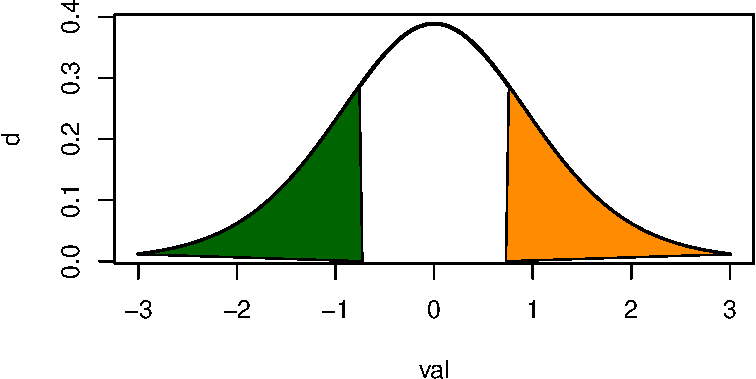
\includegraphics[keepaspectratio]{quantile-pvalue-ic_files/figure-pdf/unnamed-chunk-3-1.pdf}}

L'area sottesa alla curva evidenziata in verde è:

\[\int_{-\infty}^{-t_0} f_T(t \mid \theta) \, dt\] e si ottiene con il
codice:

\begin{Shaded}
\begin{Highlighting}[]
\FunctionTok{pt}\NormalTok{(mytest}\SpecialCharTok{$}\NormalTok{statistic, }\DecValTok{10}\NormalTok{)}
\end{Highlighting}
\end{Shaded}

\begin{verbatim}
        t 
0.2416378 
\end{verbatim}

L'area sottesa alla curva evidenziata in arancione è:

\[\int_{+t_0}^{+\infty} f_T(t \mid \theta) \, dt\]

e si ottiene con il codice:

\begin{Shaded}
\begin{Highlighting}[]
\DecValTok{1}\SpecialCharTok{{-}}\FunctionTok{pt}\NormalTok{(}\FunctionTok{abs}\NormalTok{(mytest}\SpecialCharTok{$}\NormalTok{statistic), }\DecValTok{10}\NormalTok{) }\CommentTok{\# il valore assoluto è necessario perché la}
\end{Highlighting}
\end{Shaded}

\begin{verbatim}
        t 
0.2416378 
\end{verbatim}

\begin{Shaded}
\begin{Highlighting}[]
                               \CommentTok{\# statistica test è negativa}
\end{Highlighting}
\end{Shaded}

Ma sono uguali per la simmetria della distribuzione di probabilità di
riferimento. Per il calcolo del p-value del test quindi si può applicare
il codice:

\begin{Shaded}
\begin{Highlighting}[]
\DecValTok{2}\SpecialCharTok{*}\NormalTok{(}\DecValTok{1}\SpecialCharTok{{-}}\FunctionTok{pt}\NormalTok{(}\FunctionTok{abs}\NormalTok{(mytest}\SpecialCharTok{$}\NormalTok{statistic), }\DecValTok{10}\NormalTok{))}
\end{Highlighting}
\end{Shaded}

\begin{verbatim}
        t 
0.4832757 
\end{verbatim}

che è uguale al valore del \(p\) value ottenuto mediante l'applicazione
del test:

\begin{Shaded}
\begin{Highlighting}[]
\NormalTok{mytest}\SpecialCharTok{$}\NormalTok{p.value}
\end{Highlighting}
\end{Shaded}

\begin{verbatim}
[1] 0.4832757
\end{verbatim}

\subsection{Ipotesi monodirezionale
sinistra}\label{ipotesi-monodirezionale-sinistra}

\pandocbounded{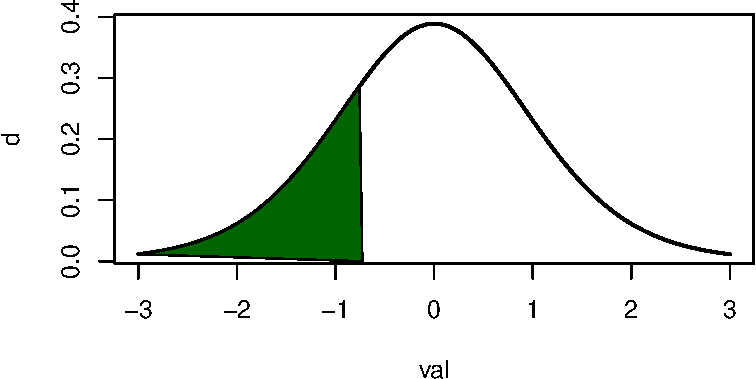
\includegraphics[keepaspectratio]{quantile-pvalue-ic_files/figure-pdf/unnamed-chunk-8-1.pdf}}

L'area sottesa alla curva evidenziata in verde è:

\[\int_{-\infty}^{-t_0} f_T(t \mid \theta) \, dt\]

che si ottiene con il codice:

\begin{Shaded}
\begin{Highlighting}[]
\FunctionTok{pt}\NormalTok{(mytest}\SpecialCharTok{$}\NormalTok{statistic, }\DecValTok{10}\NormalTok{)}
\end{Highlighting}
\end{Shaded}

\begin{verbatim}
        t 
0.2416378 
\end{verbatim}

che infatti è coerente con il valore del p-value ottenuto per il test a
una coda sinistra:

\begin{Shaded}
\begin{Highlighting}[]
\NormalTok{testmonosx }\OtherTok{=} \FunctionTok{t.test}\NormalTok{(x, }\AttributeTok{mu =}\NormalTok{ mu0,}
       \AttributeTok{alternative =} \StringTok{"less"}\NormalTok{) }
\NormalTok{testmonosx}\SpecialCharTok{$}\NormalTok{p.value}
\end{Highlighting}
\end{Shaded}

\begin{verbatim}
[1] 0.2416378
\end{verbatim}

\subsection{Ipotesi monodirezionale
destra}\label{ipotesi-monodirezionale-destra}

\pandocbounded{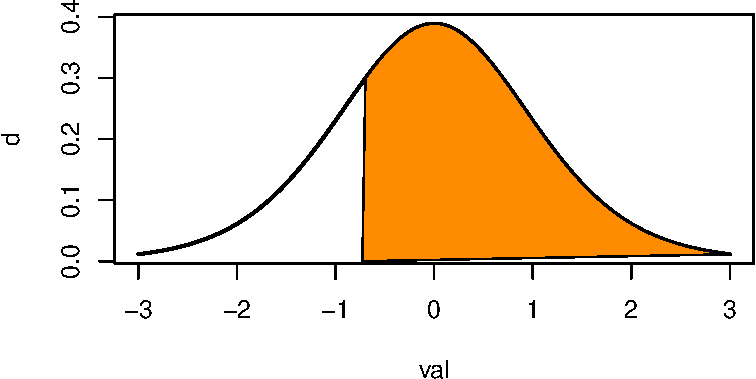
\includegraphics[keepaspectratio]{quantile-pvalue-ic_files/figure-pdf/unnamed-chunk-11-1.pdf}}

L'area sottesa alla curva evidenziata in arancione è:

\[\int_{t_0}^{+\infty} f_T(t \mid \theta) \, dt\]

e si ottiene con il codice:

\begin{Shaded}
\begin{Highlighting}[]
\DecValTok{1}\SpecialCharTok{{-}}\FunctionTok{pt}\NormalTok{(mytest}\SpecialCharTok{$}\NormalTok{statistic, }\DecValTok{10}\NormalTok{) }\CommentTok{\# il valore assoluto è necessario perché la}
\end{Highlighting}
\end{Shaded}

\begin{verbatim}
        t 
0.7583622 
\end{verbatim}

\begin{Shaded}
\begin{Highlighting}[]
                               \CommentTok{\# statistica test è negativa}
\end{Highlighting}
\end{Shaded}

che infatti è coerente con il valore del p-value ottenuto per il test a
una coda destra:

\begin{Shaded}
\begin{Highlighting}[]
\NormalTok{testmonodx }\OtherTok{=} \FunctionTok{t.test}\NormalTok{(x, }\AttributeTok{mu =}\NormalTok{ mu0,}
       \AttributeTok{alternative =} \StringTok{"greater"}\NormalTok{) }
\NormalTok{testmonodx}\SpecialCharTok{$}\NormalTok{p.value}
\end{Highlighting}
\end{Shaded}

\begin{verbatim}
[1] 0.7583622
\end{verbatim}

\section{\texorpdfstring{Calcolo del t critico
\(t_c\)}{Calcolo del t critico t\_c}}\label{calcolo-del-t-critico-t_c}

Il valore del critico viene definito a seconda di:

\begin{itemize}
\tightlist
\item
  \(\alpha\)
\item
  Ipotesi alternativa
\item
  Gradi di libertà della distribuzione \(t\) di Student
\end{itemize}

Per il loro calcolo, va usata la funzione \texttt{qt(p,\ df)}, dove
\(p\) è il valore di probabilità definito da \(\alpha\) in base al tipo
di ipotesi alternativa (mono vs.~bidirezionale) e \(df\) sono i gradi di
libertà legati alla distribuzione.

\subsection{Ipotesi bidirezionale}\label{ipotesi-bidirezionale-1}

Per \(\alpha = .05\) e ipotesi bidirezionale, con la distribuzione di
riferimento con \(gdl = 10\), \(t_c\) si ottiene con:

\phantomsection\label{annotated-cell-15}%
\begin{Shaded}
\begin{Highlighting}[]
\FunctionTok{qt}\NormalTok{(.}\DecValTok{025}\NormalTok{, }\AttributeTok{df =} \DecValTok{10}\NormalTok{) }\hspace*{\fill}\NormalTok{\circled{1}}
\FunctionTok{qt}\NormalTok{(.}\DecValTok{975}\NormalTok{, }\AttributeTok{df =} \DecValTok{10}\NormalTok{) }\hspace*{\fill}\NormalTok{\circled{2}}
\end{Highlighting}
\end{Shaded}

\begin{description}
\tightlist
\item[\circled{1}]
Restituisce il valore del quantile che è preceduto dallo .025 di
probabilità
\item[\circled{2}]
Restituisce il valore del quantile che è preceduto dallo .975 di
probabilità
\end{description}

\begin{verbatim}
[1] -2.228139
[1] 2.228139
\end{verbatim}

\subsection{Ipotesi monodirezionale
sx}\label{ipotesi-monodirezionale-sx}

Per \(\alpha = .05\) e ipotesi monodirezionale sx, con la distribuzione
di riferimento con \(gdl = 10\), \(t_c\) si ottiene con:

\begin{Shaded}
\begin{Highlighting}[]
\FunctionTok{qt}\NormalTok{(.}\DecValTok{025}\NormalTok{, }\AttributeTok{df =} \DecValTok{10}\NormalTok{) }
\end{Highlighting}
\end{Shaded}

\begin{verbatim}
[1] -2.228139
\end{verbatim}

\subsection{Ipotesi monodirezionale
dx}\label{ipotesi-monodirezionale-dx}

Per \(\alpha = .05\) e ipotesi monodirezionale dx, con la distribuzione
di riferimento con \(gdl = 10\), \(t_c\) si ottiene con:

\begin{Shaded}
\begin{Highlighting}[]
\FunctionTok{qt}\NormalTok{(.}\DecValTok{975}\NormalTok{, }\AttributeTok{df =} \DecValTok{10}\NormalTok{) }
\end{Highlighting}
\end{Shaded}

\begin{verbatim}
[1] 2.228139
\end{verbatim}

\subsection{In generale}\label{in-generale}

Cambiando i valori di probabilità \(p\) si esplicita il valore di
\(\alpha\) di riferimento:

\phantomsection\label{annotated-cell-18}%
\begin{Shaded}
\begin{Highlighting}[]
\FunctionTok{qt}\NormalTok{(.}\DecValTok{90}\NormalTok{, }\DecValTok{10}\NormalTok{) }\hspace*{\fill}\NormalTok{\circled{1}}
\FunctionTok{qt}\NormalTok{(.}\DecValTok{10}\NormalTok{, }\DecValTok{10}\NormalTok{) }\hspace*{\fill}\NormalTok{\circled{2}}
\end{Highlighting}
\end{Shaded}

\begin{description}
\tightlist
\item[\circled{1}]
\(\alpha = .10\) e ipotesi monodirezionale destra
\item[\circled{2}]
\(\alpha = .10\) e ipotesi monodirezionale sinistra
\end{description}

\begin{verbatim}
[1] 1.372184
[1] -1.372184
\end{verbatim}

\section{Intervallo di confidenza}\label{intervallo-di-confidenza}

L'intervallo di confidenza viene calcolato come:

\[IC_p = \bar{x}\pm t_c * \sigma_{\bar{x}}\] Dove \(p\) è la probabilità
determinata come \(1 -\alpha\), \(t_p\) è il valore di \(t\) critico per
\(\alpha\) (con hp bidirezionale) e \(\sigma_{\bar{x}}\) è l'errore
standard ottenuto come:

\[\sigma_{\bar{x}} = \dfrac{\bar{x} - \mu_0}{\sqrt{var(x)/N}}\] Ad
esempio, per calcolare l'intervallo di confidenza al 90\% (quindi
\(\alpha = .10\)) sui dati campionari di prima:

\phantomsection\label{annotated-cell-19}%
\begin{Shaded}
\begin{Highlighting}[]
\NormalTok{mx }\OtherTok{=} \FunctionTok{mean}\NormalTok{(x) }\hspace*{\fill}\NormalTok{\circled{1}}
\NormalTok{se }\OtherTok{=} \FunctionTok{sqrt}\NormalTok{(}\FunctionTok{var}\NormalTok{(x)}\SpecialCharTok{/}\FunctionTok{length}\NormalTok{(x)) }\hspace*{\fill}\NormalTok{\circled{2}}
\NormalTok{tc }\OtherTok{=} \FunctionTok{qt}\NormalTok{((}\DecValTok{1}\FloatTok{{-}.10}\SpecialCharTok{/}\DecValTok{2}\NormalTok{), }\AttributeTok{df =} \DecValTok{10}\NormalTok{) }\hspace*{\fill}\NormalTok{\circled{3}}
\NormalTok{mx }\SpecialCharTok{{-}}\NormalTok{ tc}\SpecialCharTok{*}\NormalTok{se }\hspace*{\fill}\NormalTok{\circled{5}}
\NormalTok{mx }\SpecialCharTok{+}\NormalTok{ tc}\SpecialCharTok{*}\NormalTok{se }\hspace*{\fill}\NormalTok{\circled{6}}
\end{Highlighting}
\end{Shaded}

\begin{description}
\tightlist
\item[\circled{1}]
Media di \(x\)
\item[\circled{2}]
Standard error
\item[\circled{3}]
Quantile inferiore di \(t\)
\item[\circled{5}]
Limite inferiore dell'intervallo
\item[\circled{6}]
Limite superiore dell'intervallo
\end{description}

\begin{verbatim}
[1] 4.414237
[1] 12.38424
\end{verbatim}




\end{document}
